 \chapter{Modélisation des circonstances factuelles par catégorisation non supervisé de documents}
\label{chap:similarite}

%\epigraph{Le plus important, c'est d'avoir un langage métaphorique ; car c'est le seul mérite qu'on ne puisse emprunter à un autre et qui dénote un esprit naturellement bien doué ; vu que, bien placer une métaphore, c'est avoir égard aux rapports de ressemblance.}{Aristote, Poétique}
% 

\section{Introduction}
\label{sec:similarite:introduction}
Les circonstances factuelles définissent les contextes possibles dans lesquels une catégorie de demande peut être formulée. Les analyses descriptives ou prédictives ne prennent sens que lorsqu'elles sont appliquées à un ensemble de décisions aux circonstances similaires. Par exemple, il serait imprudent de considérer toutes les décisions pour analyser les chances d'acceptation d'une demande de dommages-intérêts fondée sur l'\og article 700 du code de procédure civile \fg{} en cas de trouble de voisinage. Les taux d'acceptation ou de rejet peuvent être différents entre des affaires de licenciement et celles portant sur les troubles anormaux du voisinage, et même plus spécifiquement entre les troubles de voisinage entre particulier et entreprises. % (par exemple: chantier de construction), ou simplement entre particuliers (par exemple: troubles sonores). 
 Il serait préférable de travailler uniquement avec des décisions similaires à la situation d'intérêt. L'identification des circonstances factuelles devient donc une étape préalable indispensable à l'analyse du résultat. Malheureusement, les circonstances sont très diverses et quasi infinies pour être identifier par classification supervisée à l'aide d'annotation manuelle d'exemples comme dans les chapitres précédent. Il est donc plus indiquer d'adopter une approche non-supervisée capable modéliser les circonstances factuelles à partir d'un corpus de documents d'une même catégorie de demande. Plus précisément, la méthode doit construire des sous-ensembles de décisions selon qu'elles traitent de contextes similaires.  Les objectifs de ce chapitre sont d'expérimenter des algorithmes  de regroupement (\textit{clustrering}) et des métriques de similarité. Il démontre aussi qu'une distance entraînée  sur des documents d'une catégorie de demande permet de mieux mesurer la (dis-) similarité sémantique définie par les circonstances factuelles.

%\section{Formulation du Problème}
%\label{sec:similarite:probleme}

\section{Regroupement non-supervisé de documents}
\label{sec:similarite:biblio}

Cette section fait une synthèse bibliographique des différents aspects rentrant dans la conception d'un système de regroupement de documents. Elle aborde principalement le choix de l'algorithme, la définition d'une mesure de similarité adéquate, la représentation des documents, la détermination du nombre de {clusters}, et l'évaluation du regroupement généré.

L'ensemble des $N$ documents est noté $\mathcal{D}$. Tout document $d \in \mathcal{D}$ est une séquence de mots $d=(d_1, d_2, \dots, d_{\setsize{d}})$, où $d_i$ est le mot à la position $i$ dans $d$. Sa représentation vectorielle est notée $\vec{d}=(\vec{d}_1, \vec{d}_2, \dots, \vec{d}_m)$. Pour un modèle vectoriel TF-IDF de vocabulaire $T = (t_1, t_2, \dots, t_m)$, $\vec{d}_i = w(t_i,d)$ est le poids du terme $t_i \in T$ dans le texte $d$ ({cf. \ref{sec:quanta:classification}}). Le regroupement obtenu est un ensemble de clusters $C = \lbrace C_1, C_2, \cdots, C_K \rbrace$, $K$ étant le nombre de clusters formés.

\subsection{Algorithmes de regroupement non-supervisé}

Le regroupement de documents a pour objectif  d'identifier, sans supervision\footnote{Sans utiliser des exemples annotés.}, une structure pertinente (pour le domaine expert) dans l'ensemble $\mathcal{D}$ en construisant des groupes représentants des catégories inconnues au départ. Ces groupes, appelés clusters, peuvent être disjoints ou se chevaucher, et plates ou hiérarchiques suivant les contraintes du domaine expert. L’algorithme à utiliser dépend généralement de la forme qu’on souhaite donner à l’organisation. 

\subsubsection{Partitionnement disjoint}
Pour réaliser des partitions distinctes\footnote{Chaque document n'appartient qu'à un seul cluster.} (\textit{hard clustering}), des algorithmes tels que celui des K-moyennes \citep{forgey1965kmeans} et celui des \textit{K-medoïdes} \citep{kaufman1987kmedoids} seront préférés \citep{balabantaray2015kmeanskmedoids}. Ces deux algorithmes fonctionnent de manière similaire, et nécessitent que le nombre $K$ de clusters soient prédéfini. Ils commencent par une définition aléatoire de $K$ centres initiaux de clusters (centroïdes) et l'affectation des différents documents au cluster dont le centre est le plus proche. S'en suit une boucle dans laquelle le centroïde est recalculé (le point à distance totale minimale avec les membres du cluster) et les documents sont réaffectés chacun au cluster dont le centroïde est le plus proche. L'algorithme s'arrête si aucune amélioration n'est plus observée, ce qui se traduit soit par l'atteinte d'une valeur minimale prédéfinie de l'erreur de \textit{clustering}\footnote{Somme des distances au carré entre les points et leur centre respectif.} ou d'une mesure d'évaluation non supervisée (\ref{sec:similarite:biblio:unsupeval}). La différence entre l'algorithmes des K-moyennes et celui des \textit{K-medoïdes} tient principalement au fait que les centroïdes du premier ne sont pas nécessairement des points (documents) de l'ensemble d'origine, mais des points moyennes des représentations vectorielles des membres du cluster, contrairement à l'algorithme des \textit{K-medoïdes} qui ne considère que les documents originaux qui ont une distance minimale à tous les documents dans leur cluster. Cette différence donne l'avantage au \textit{K-medoïdes} de ne pas dépendre d'une représentation vectorielle nécessaire au calcul de la moyenne, mais elle a aussi l'inconvénient d'augmenter sa complexité en temps  car il faut calculer et stocker la distance entre toutes les paires de documents. Il existe plusieurs autres algorithmes de regroupement disjoint dont le principe de fonctionnement est différent de celui des K-moyennes. Par exemple, l'algorithme DBSCAN (\textit{Density-based spatial clustering of applications with noise}) \citep{ester1996dbscan}  ne prend pas en paramètre le nombre de clusters à construire. Il est défini sur le concept de régions de densité caractérisées par la distance minimale $\epsilon$ autorisée entre deux points d'une même région, et le nombre maximal de points qui doivent être dans le voisinage de rayon $\epsilon$ d'un point pour que ce voisinage soit une région de densité (le point central est appelé "point noyau" (\textit{core point}). Le principe du DBSCAN est de construire les clusters successivement en reliant les régions (voisinages) dont les noyaux sont à distance plus ou moins inférieure à $\epsilon$. Les points qui sont seul dans leur cluster sont qualifiés d'\textit{outliers}. 
% amélioration par réduction de dimension
En outre, le regroupement spectral est une autre méthode efficace de regroupement qui effectue préalablement une réduction de dimensions à l'aide du spectre de la matrice de similarité $M \in \mathbb{R}^{N \times N}$ \footnote{$M_{ij}$ est la mesure de la similarité entre les points (documents) $d_i$ et $d_j$ du corpus $D$.} des données  avant d'appliquer un algorithme traditionnel comme celui des K-moyennes. Les dimensions du nouvel espace sont définies par les vecteurs propres de la matrice Laplacienne $L$ de $M$ \citep{shi2000spectralClustering, von2007tutorialSpectralClustering} qui peut être normalisée ($L = T^{-1/2}(T-S)T{-1/2}$) ou pas ($L = T - M$), $T$ étant la matrice diagonale déduite de $M$ i.e. $T_{ii} = \sum\limits_j M_{ij}$. 

Il est aussi possible d'utiliser les arbres de décision pour améliorer les résultats des K-moyennes. En effet, les forêts aléatoires \citep{breiman2001randomforest} permettent d'estimer la similarité entre deux points. Le principe consiste à générer un ensemble de $n$ points synthétiques, et d'entraîner une forêt aléatoire à une classification binaire supervisée avec les points originaux considérés dans la classe des "originaux" et les données synthétiques dans la seconde classe des "synthétiques" \citep{afanador2016unsupervisedrandomforest}. Une forêt aléatoire étant un ensemble d'arbres de décision (classification) construit sur des parties de l'ensemble d'apprentissage duquel on a retiré une ou plusieurs variables prédictives, la similarité entre 2 points est la proportion d'arbres dans lesquels ces points se trouvent dans le même nœud feuille. Cette métrique "apprise" peut-être par la suite utilisée dans un algorithme de regroupement classique comme les K-moyennes.

%\textcolor{red}{Random Forest - processus de construction: \url{https://onlinelibrary.wiley.com/doi/pdf/10.1002/cem.2790}}

%L'application de ces différents algorithmes aux documents n'est généralement basé que sur les statistiques d'occurrence des termes, et par conséquent les thématiques abordées dans les documents ne sont pas bien prise en compte, surtout que l'élimination des \og mots vides \fg{} (\textit{stop words}) peut laisser les deux documents sans sinon très peu de mots en commun \cite{kusner2015wordmoverdist}. \citet{xie2013MGCTM} démontrent empiriquement que l'intégration de la  modélisation thématique (\textit{topic modeling}) au clustering de documents améliore significativement les résultats. Cette intégration des modèles thématiques dans le clustering de documents peut être réalisée de multiples façons, mais deux méthodes semblent être les plus efficaces:
%\begin{enumerate}
%	\item l'intégration naïve \citep{lu2011kmeansLDApLSA} qui consiste à inférer $K$ thèmes à l'aide d'un algorithme comme le PLSA (aAnalyse sémantique probabiliste latente) \citep{hofmann1999PLSA} ou le LDA (allocation de Dirichlet latente)\citep{blei2003lda}, puis de considérer pour chaque document le thème $j \in [1..K]$ qui a la probabilité $\theta_j$ la plus élevé dans ce document suivant la distribution $\theta$ de probabilité des thèmes dans ce document; le thème choisi $j$ représente le cluster du document;
%	\item le modèle thématique multi-grain de clustering (\textit{multi-grain clustering topic model}) ou MGCTM proposé par \citet{xie2013MGCTM}, dont l'objectif est d'inférer de manière jointe les clusters et le modèle thématique.
%\end{enumerate}

\subsubsection{Regroupement avec chevauchements}

Lorsque des chevauchements sont observables entre clusters (un document peut faire partie de plusieurs groupes à la fois), chaque objet peut être affecté partiellement à chaque cluster grâce à la notion de degré d'appartenance (\textit{membership degree}) entre un point $x_i \in X$ et le cluster $j \in [1..K]$ estimé par une fonction $u_{ij}$  \citep{baraldi1999surveyfuzzyclstering}. Il est par conséquent préférable d'employer des algorithmes de partitionnement "mou" comme l'algorithme des c-moyennes flou (FCM) \citep{bezdek1984fcm, hathaway1989fuzzycmeans}, ou le fuzzy c-Medoids (FDMdd) \citep{krishnapuram2001fuzzycmedoids}, ou la version améliorée IFKM (\textit{improved fuzzy K-medoids})\citep{sabzi2011fuzzykmedoids}.  Le principe de ces algorithmes consiste en deux étapes principales \citep{sabzi2011fuzzykmedoids}: 

\begin{enumerate}
 \item l'estimation des degrés d'appartenance de chaque instance $x_i \in X$ à chaque cluster $j \in [1..K]$ de centroïde $z_j$ réalisée par la minimisation de la fonction objective $P(X,Z) = \sum\limits_{i=1}^{n}\sum\limits_{j=1}^{k} \left[u_{ij}r(x_i,z_j)\right]$ \citep{krishnapuram2001fuzzycmedoids}  améliorée par \citet{sabzi2011fuzzykmedoids} en:
 \[P(X,Z) = \sum\limits_{i=1}^{n}\sum\limits_{j=1}^{K} \left[u_{ij}r(x_i,z_j)\right] + \lambda \sum\limits_{i=1}^{n}\sum\limits_{j=1}^{K} \left[ u_{ij}\log_2(u_{ij}) \right] \]
 \[s.c. \sum\limits_{j=1}^{k} u_{ij} = 1\]
 \[0 \leq u_{ij} < 1\]
 
 dont la valeur approximative généralement utilisée de la solution est \[u_{ij} = \frac{\exp\left(\frac{-r(x_i,z_j)}{\lambda}\right)}{\sum_{l=1}^{k}\exp\left(\frac{-r(x_l,z_j)}{\lambda}\right)},\] $r(x_i,z_j)$ étant la mesure de dis-similarité (distance) entre $x_i$ et  $z_j$;
 \item la détermination des nouveaux centres de clusters qui s'effectue toujours par la moyenne des membres du cluster chez le fuzzy c-means, mais par le choix de l'objet $x_q$ qui optimise la somme des distances de cet objet aux autres membres pondérée chacune par le degré d'appartenance de ces autres membres: \[\forall j \in  \left[1\twodots k \right], q = \argmin\limits_{1 \leq l < s_j} \sum\limits_{l=1}^{s_j} \left[u_{lj}r(x_l,z_j)\right]\] $s_j$ étant le nombre de membres du cluster $j$.
\end{enumerate}
 Ainsi l'objectif de l'entraînement des algorithmes de regroupement flou est double: déterminer les valeurs optimales de la matrice $U$ des degrés d'appartenance et l'ensemble $Z$ des centroïdes. 
 
 Les regroupements avec chevauchement sont intéressants parce qu'il est possible qu'une décision traite de plusieurs circonstances factuelles.
%\textcolor{red}{A COMPLETER!!!!!!!!!!}
%Pour des regroupements hiérarchiques, des algorithmes comme celui du clustering par agglomération (\textit{agglomeration clustering}) sont mieux indiqués. Le principe du clustering par agglomération est de ...
%si les chevauchements sont négligeables ou n'existent pas, ou bien si la structure hiérarchique permettrait de mieux expliquer et distinguer les différences inter-groupes et les ressemblances intra-groupes. Nous souhaitons organiser des décisions de justices en fonction des circonstances factuelles auxquelles ces documents sont liés.  On pourrait par exemple faire une restriction des données aux cas où chaque document n’appartient qu’à une classe et proposer un système de clustering disjoint.

%\subsubsection{Limites des algorithmes de clustering}
%nombre prédéfini de clusters, initialisation aléatoire des centroïdes menant à des clusters différents entre plusieurs exécution \citep{sabzi2011fuzzykmedoids}. Nous noterons aussi la dépendance à la métrique de similarité.
%Algorithme kmeans + kmédoids pour les documents: https://pdfs.semanticscholar.org/a46f/efdb64a01d1e6390c8212d881b9c4414ffbf.pdf


\subsection{Métriques de dis-similarité (distances)}
\label{sec:similarite:distances}
Les algorithmes de regroupement dépendent de la distance utilisée qui doit être bien choisie pour que les regroupements révèlent au mieux la sémantique visée.
 Une métrique de dis-similarité $Dis$ est une fonction réelle d'une paire $(d,d')$ qui mesure le degré de dis-similarité entre $d$ et $d'$  en satisfaisant aux propriétés suivantes $\forall d,d',d'' \in \mathcal{D}$ \citep{wang2015distancemetriclearningsurvey}:
\begin{enumerate}
\item $Dis(d,d') \geq 0$ ("non-négativité")
\item $Dis(d,d') = 0  \Leftrightarrow d = d'$ (identité discernable)
\item $Dis(d,d') = Dis(d', d)$ (symétrie)
\item $Dis(d,d'') \leq Dis(d,d') + Dis(d',d'')$ (inégalité triangulaire) \label{enum:sim:ineq-tri}
\end{enumerate}


La métrique peut être normalisée ($\forall (d,d') \in \mathcal{D} \times \mathcal{D};  0 \leq Dis(d,d') \leq 1$), à l'instar de la distance basée sur la similarité cosinus normalisée et celle de Jaccard. Dans ce cas, la relation entre la similarité $Sim$ et la dis-similarité $Dis$ est définie par $Sim(d,d') = 1 - Dis(d,d')$.
%On parle de \textbf{pseudo-métrique} lorsque la condition \ref{enum:sim:ineq-tri} n'est pas satisfaite.

 Il existe de nombreuses métriques de similarité généralement expérimentées pour le regroupement de textes \citep{huang2008similarityTextClustering, vijaymeena2016surveySim, afzali2018SimKmeans}:
\begin{itemize}
	\item Les distances de Minkowski de forme générale $Dis(d,d') = \norm{\vec{d} - \vec{d'}}_{Lp} = \sqrt[p]{\sum\limits_{i=1}^m \vert \vec{d}_i - \vec{d}_i \vert ^p}$, dont font partie la distance euclidienne $Dis_{euclidienne}$ ($p=2$) et la distance de Manhattan $Dis_{manhattan}$ ($p=1$).
	\item La distance de \citet{bray1957distance-braycurtis}: $Dis_{braycurtis}(d,d') = \frac{\sum\limits_{i=1}^m \vert \vec{d}_i - \vec{d'}_i \vert}{\sum\limits_{i=1}^m \vert \vec{d}_i + \vec{d'}_i \vert}$\citep{huang2008similarityTextClustering}.
	\item La similarité cosinus est basée sur la mesure de l'angle entre $\vec{d}$ et $\vec{d'}$ par la formule: $Sim_{cos}(d,d') = \frac{\vec{d}^t\vec{d'}}{\norm{\vec{d}}\norm{\vec{d'}}}$.
	Pour un modèle vectoriel du type TF-IDF, cette formulation considère que tous les termes du vocabulaire $T$ définissant le modèle vectoriel, sont différents et ne partagent aucune relation. \citet{sidorov2014softcosine} la corrigent en proposant la fonction \textit{soft-cosine} en introduisant une matrice $S = {S_{ij}}_{1\leq i,j \leq m}$ de similarité entre  termes: 
	
	$Sim_{soft-cos}(d,d')= \frac{{\vec{d}}^T\cdot S\cdot \vec{d'}}{\sqrt{{\vec{d}}^T\cdot S\cdot \vec{d'}}\cdot \sqrt{\vec{d'}^T\cdot S\cdot \vec{d'}}} = \frac{\sum\limits_{1\leq i,j \leq m}s_{ij}\vec{d}_i\vec{d'}_j}{\sqrt{\sum\limits_{1\leq i,j \leq m}s_{ij}\vec{d}_i\vec{d}_j}\sqrt{\sum\limits_{1\leq i,j \leq m}s_{ij}\vec{d'}_i\vec{d'}_j}}$,
	
	où $S$, la matrice de similarité entre les termes, peut être calculée à partir de n'importe quelle métrique comme la distance d'édition de Levenshtein (similarité lexicale) \citep{sidorov2014softcosine},  la similarité cosinus entre  plongements lexicaux \citep{charlet2017simbow_acl, charlet2017simbow_tal}, ou la similarité WordNet.
	
	La fonction cosinus  étant comprise entre -1 et +1, sa forme normalisée s'écrit  $\overline{Sim}_{cos}(d,d') = \frac{Sim_{cos}(d,d') + 1}{2}$, d'où la distance $Dis_{cos}(d,d') = 1 - \overline{Sim}_{cos}(d,d')$.
	
	\item Le coefficient similarité de \cite{jaccard1901similarite-jaccard}: $Sim_{Jaccard}(d,d') = \frac{\vec{d}^T\vec{d'}}{\norm{\vec{d}}^2+\norm{\vec{d'}}^2 - \vec{d}^T\vec{d'}}$ \citep{huang2008similarityTextClustering} qui, étant normée, donne la distance $Dis_{jaccard}(d,d') = 1-Sim(d,d')$.
	%\item Le coefficient similarité de Dice: $Sim_{Dice}(x,x') = \frac{2\cdot \vert tok(x) \cap tok(x') \vert}{\vert tok(x) \vert + \vert tok(x')} $
	\item La similarité basée sur le coefficient de corrélation de Pearson est calculée par \citep{huang2008similarityTextClustering}:
	
	\[Sim_{pearson}(d,d') = \frac{ \sum\limits^m_{i=1} \vec{d}_i \cdot \vec{d'}_i - TF_d\cdot TF_{d'}}{\sqrt{[m \sum\limits^m_{i=1} \vec{d'}_i^2 - TF^2_d][m \sum\limits^m_{i=1} \vec{d'}_i^2 - TF^2_{d'}]}}\]
avec $TF_d = \sum\limits^m_{i=1} \vec{d}_i$. Sa distance est déduite par:

$Dis_{pearson}(d,d') =
\left\{ \begin{array}{ll}
1 - Sim_{pearson}(d,d') & \text{si } Sim_{pearson}(d,d') \geq 0 \\
\vert Sim_{pearson}(d,d') \vert & \text{si } Sim_{pearson}(d,d') < 0.
\end{array}
\right.$
%	\item Distance de la divergence moyenne de Kullback-Leibler considère un document comme une distribution de probabilité de termes, et mesure donc la similarité entre deux distributions: 
%	\[Dis_{avgKL}(x,x') = \sum\limits_{i=1}^m\big(\pi_1 \cdot D(w(t_i,x) \vert\vert w_t) + \pi_2 \cdot D(w(t_i,x') \vert\vert w_t) \big)\]
%	avec $\pi_1 = \frac{w(t_i,x)}{w(t_i,x) + w(t_i,x')}$, $\pi_2 = \frac{w(t_i,x')}{w(t_i,x) + w(t_i,x')}$, $D(a \vert\vert b) = a\cdot  \log_2(\frac{a}{b})$, et $w_t = \pi_1 \cdot w(t_i,x) + \pi_2 \cdot w(t_i,x')$
%	\item Okapi BM25 est une métrique de similarité généralement utilisée en recherche d'information pour calculer un score de pertinence d'un document D par rapport à une requête Q: 
%	\[Sim_{BM25}(Q,D) = \sum\limits_{w \in Q \cap D} \left( \frac{(k_3+1) \cdot c(w, Q)}{k_3 + c(w, Q)} \cdot f(w,D) \cdot \log \frac{N+1}{df(w) + 0.5)}\right),\]
%	\[\text{avec } f(w,D) = \frac{(k_1+1)\cdot c(w,D)}{k_1(1-b+b\frac{\vert D \vert}{avgdl})} = \frac{(k_1+1)\cdot c'(w,D)}{k_1 + c'(w,D)},\] où $c'(w,D) = \frac{c(w,D)}{1-b+b\frac{\vert D \vert}{avgdl} }$. $c'(w,D)$ pouvant approcher 0 pour des documents très longs, \citet{Lv2011BM25L} propose BM25L, une formulation plus robuste à la longueur des documents obtenue en remplaçant $f(w,D)$ par :
%	\[
%	f'(w,D) =
%	\left\{ \begin{array}{ll}
%	\frac{(k_1+1)\cdot (c'(q,D)+\delta)}{k_1+ (c'(w,D) + \delta)} & \text{si } c'(w,D) > 0 \\
%	0 & \text{si } sinon
%	\end{array}
%	\right.
%	\]
	\item \og La distance du déménageur de mot \fg{} (\textit{word mover's distance - WMD}) \citep{kusner2015wordmoverdist} est une méthode dont l'objectif est similaire au notre, i.e. inclure la similarité sémantique entre les paires de mots de deux documents dans l'estimation de la distance entre ces derniers. En effet, elle est la solution optimale du problème de transport suivant \footnote{Valeur minimale du cout cumulatif pondéré nécessaire pour déplacer  tous les mots de $d$ à $d'$ i.e. transformer $d$ en $d'$.}:
	
	\begin{equation*}
	\begin{aligned}
Dis_{wmd}(d, d') = 	& \min\limits_{T>0}
	& & \sum\limits_{i,j=1}^m T_{ij} c(i,j) \\
	& \text{s.c.}
	& & \sum\limits_{j=1}^m T_{ij} = \vec{d}_i, \forall i \in {1, \dots, m} \\
	& 
	& & \sum\limits_{i=1}^m T_{ij} = \vec{d'}_j, \forall j \in {1, \dots, m}	
	\end{aligned}
	\end{equation*} 
	
	$m$ est le nombre de mots considérés; $T$ est une matrice dont $T_{ij}$ est interprété comme étant la quantité du mot $i$ de $d$ qui est va au mot $j$ dans $d'$ ("voyage"). $c(i,j)$ est la distance euclidienne entre les vecteurs des mots $i$ et $j$; $\vec{d}_i$ et $\vec{d'}_j$ sont les composantes aux mots $i$ et $j$ resp. des vecteurs normalisés sac-de-mots de $d$ et $d'$ reesp. i.e. $\vec{d}_i = \frac{compte(i, d)}{\sum\limits_{k=1}^m compte(k, d)}$, où $compte(i, d)$ est le nombre d'occurrences du mot $i$ dans $d$.
	
\end{itemize}


%Par contre, les métriques {apprises} sont définies à partir de connaissances des données labellisées. Ces métriques sont apprises pour répondre à la difficulté d'identifier la métrique statique appropriée pour un problème. L'apprentissage exploite un corpus préalablement annoté. L'apprentissage peut être supervisé si l'annotation du corpus consiste soit en classifiant des documents\footnote{Organisation des documents d'entraînement en des groupes aux labels prédéfinis.} \citep{weinberger2005LMNN}, soit en affectant des mesures de similarité à des paires de documents \citep{bibid}.  Un apprentissage semi-supervisé typique utilise des données annotées par jugements relatifs sur des pairs ou triplets de documents. Les contraintes de couples consistent en deux ensembles, l'un comprenant des couples de documents qui doivent être similaires, et l'autre contenant des couples de documents dis-similaires. Les contraintes de triplets consistent à définir pour un triplet de documents $(x_1,x_2,x_3)$ une comparaison de degré de similarité entre les paires (par exemple, $x_1$ est plus similaire à $x_2$ qu'à $x_3$). La métrique apprise est néanmoins une véritable métrique à valeur réelle positive écrite sous la forme d'une distance de Mahalanobis $f(x,y) = \sqrt{(x-y)^T M^{-1}(x-y)}$ (où $M$ est la matrice à apprendre). 
 
% L'apprentissage expérimenté dans ce chapitre est supervisé, même s'il utilise des données synthétiques. Nous supposons étant donné que les documents du corpus à \textit{clusteriser} sont tous de la même catégorie de demande, la différence entre les clusters et leur homogénéité se remarquera au niveau des faits. Par cette hypothèse, il reste un risque que d'autres types de regroupements se forment comme par exemple suivant d'autres catégories de demande co-occurrentes. Parmi les divers algorithmes réalisant un apprentissage supervisé, notons par exemple:
% \begin{itemize}
% 	\item Les plus-proches-voisins-dans-la-large-marge (LMNN) \citep{weinberger2005LMNN} plus adapté à l'annotation par classification;
% 	\item L'analyse des composants du voisinage (NCA) \citep{goldberger2005NCA};
% 	\item L'apprentissage de métrique pour la régression noyau (\textit{MLKR}) \citep{weinberger2007MLKR};
% 	\item L'analyse discriminante locale de Fisher (LFDA) \citep{sugiyama2007LFDA, } méthode supervisée (données labellisées) de réduction de dimension
% \end{itemize}

%\subsection{Représentations des textes}
%La formulation des distances exploite très souvent une représentation vectorielle des texte (cf.  \ref{sec:similarite:distances}). 


\subsection{Déterminer le nombre optimal de clusters}

%\textcolor{red}{faire un tableau des indices comme dans l'article, et comparer les combinaison indices-algo-distance}

 Au delà de l’algorithme à utiliser, le nombre $K$ approprié de clusters doit être déterminé mais pas prédéfini, puisqu'il est difficile de savoir à l'avance le nombre de groupes. Une méthode très connue est celle du \og coude \fg{}  (ou \og genou \fg{}) \citep{halkidi2001clustvalidation}, qui est basé sur le principe de base des algorithmes de partitionnement (e.g. K-moyennes) i.e. minimiser le critère d'inertie\footnote{la variance intra-cluster qui est la somme au carré des erreurs (distance d'un membre au centre).}:
\[J(K) = \sum\limits_{j=1}^K\sum\limits_{d_i \in C_j}\norm{\vec{d}_i-\overline{\vec{d}_j}}^2\]

$C_j$: ensemble des objets du cluster $j$

$\overline{\vec{d}_j}$: échantillons moyens du cluster $j$ (centre)

La méthode du coude consiste à essayer différentes valeurs consécutive de $K$ (de $K_{min}$ à $K_{max}$) puis de choisir celle qui correspond au coude de la courbe du critère d'inertie $J(K)$. Le choix de ce coude est visuel et peut être ambigu (plusieurs valeurs de $K$ sur le coude par exemple). 

La méthode de la silhouette moyenne \citep{rousseeuw1987silhouetteclusternumber} est une alternative qui consiste à choisir comme valeur optimale de $K$, celle qui maximise le critère de la largeur moyenne de la silhouette: $\overline{s_K}(C) = \frac{1}{K}\sum\limits_{i=1}^N s(d)$. La largeur $s(d)$ de la silhouette est un indice qui compare la ressemblance d'un document $d$ aux autres membres de son cluster $C_t$ par rapport à ceux d'autres clusters $C_l, l \neq t$:
\[s(d) = \frac{b(d) - a(d)}{\max\lbrace a(d),b(d)\rbrace}\]

où $a(d) = \frac{1}{\vert C_t \vert} \sum\limits_{d' \in C_t} Dis(d, d')$, et $b(d) = \min\limits_{l \neq t} \frac{1}{\vert C_l \vert} \sum\limits_{d' \in C_t} Dis(d, d')$, pour $d \in C_l$.

$K$ est optimal lorsque la largeur moyenne $\overline{s_K}(C)$ est maximale. % Salvador et Chan (2004) propose d’utiliser l’intersection des deux lignes approximant la courbe. Mais plus récemment, Zhang et al. (2016) trouvent que cette approche n’est pas appropriée pour les cas où le graphe d’évaluation n’est ni lisse, ni monotone. Ils proposent d’exploiter la courbure du graphe i.e. la valeur dont un objet géométrique s'écarte d'être plat ou droit dans le cas d'une ligne.

%Etant donné le grand nombre de méthodes existantes \citep{liu2010interclustvalidation, Amorim2015recoveringnumclust}, la majorité des votes peut être appliquée pour choisir le bon $K$ \footnote{\url{https://www.datanovia.com/en/lessons/determining-the-optimal-number-of-clusters-3-must-know-methods/}}.

%\subsection{Initialisation des centroïdes}

%\subsection{Définir une représentation appropriée pour les textes}
%\url{https://arxiv.org/pdf/1509.01626.pdf}

%\url{http://ad-publications.informatik.uni-freiburg.de/theses/Bachelor_Jon_Ezeiza_2017_presentation.pdf}


%\subsection{Labeliser les clusters}

\subsection{Validation du regroupement}
La validation d'un regroupement peut être supervisée ou non selon que des documents labellisés dans les groupes attendus (données externes) sont employées.

\subsubsection{Métriques supervisées ou mesures externes}
\label{sec:similarite:biblio:supeval}
Les métriques couramment employées mesurent la ressemblance entre deux regroupements $X = \lbrace X_1, X_2,..., X_r \rbrace$ et $Y = \lbrace Y_1,Y_2,..., Y_s \rbrace$:
\begin{itemize}
	\item l'indice ajusté par chance de Rand (\textit{ajusted Rand index} - ARI) \citep{hubert1985adjustedrandidx} corrigent l'indice de Rand (RI) \citep{rand1971randidx} pour obtenir une valeur très proche de 0.0 pour les regroupements aléatoires et exactement 1.0 lorsque les clusters sont identiques aux classes attendues. En effet, l'indice de Rand prend ses valeurs en pratique dans l'intervalle $[0.5;1]$, et a par conséquent une valeur de base très élevée. ARI est calculé à l'aide du tableau de contingence résumant les chevauchements que partagent $X$ et $Y$ (Tableau \ref{tab:similarite:tab-contingence}) par la formule: %\[ARI(Y,C) = \frac{RI(Y,C) - E_{perm}\left[RI(Y,C)\right]}{1.0 - E_{perm}\left[RI(Y,C)\right]} \]
	\[ARI(X,Y) = \frac{\sum\limits_{i,j}\binom{n_{ij}}{2} - \frac{\sum\limits_{i}\binom{a_{i}}{2}\sum\limits_{j}\binom{b_{j}}{2}}{\binom{N}{2}}}{\frac{1}{2}\big[\sum\limits_{i}\binom{a_{i}}{2}+\sum\limits_{j}\binom{b_{j}}{2}\big] - \frac{\sum\limits_{i}\binom{a_{i}}{2}\sum\limits_{j}\binom{b_{j}}{2}}{\binom{N}{2}}}, \text{ avec } \binom{n}{2} = \frac{n(n-1)}{2}.\]
	
	\begin{table}[!htb]
		\centering \small
		\begin{tabular}{|c|c|c|c|c|c|}
			\hline
			& $Y_1$    & $Y_2$    & $\cdots$ & $Y_s$    & $\sum$   \\ \hline
			$X_1$    & $n_{11}$ & $n_{11}$ & $\cdots$ & $n_{11}$ & $a_1$    \\ \hline
			$X_2$    & $n_{21}$ & $n_{21}$ & $\cdots$ & $n_{21}$ & $a_2$    \\ \hline
			$\cdots$ & $\cdots$ & $\cdots$ & $\ddots$ & $\cdots$ & $\cdots$ \\ \hline
			$X_r$    & $n_{r1}$ & $n_{r1}$ & $\cdots$ & $n_{r1}$ & $a_r$    \\ \hline
			$\sum$   & $b_1$    & $b_2$    & $\cdots$ & $b_s$    &          \\ \hline
		\end{tabular}
		\caption{Tableau de contingence des chevauchement entre les regroupements $X = \lbrace X_1, X_2, ..., X_r \rbrace$ et $Y = \lbrace Y_1, Y_2, ..., Y_s \rbrace$, $n_{i,j} = \vert X_i \cap Y_j\vert$} \label{tab:similarite:tab-contingence}
	\end{table}
ARI a des valeurs dans $[-1;1]$. Une valeur négative indique que le regroupement obtenu s'accorde moins avec l'attendu qu'un regroupement aléatoire. 
	% \item la précision du clustering (ACC) \citep{}.   \textcolor{red}{pas utilisé car nécessite de trouver le meilleur mapping entre les classes et les clusters}
	\item L'information mutuelle normalisée (NMI) \citep{kvalseth1987entropy_NMI,strehl2000nmi, vinh2010clusteringComparison} normalise l'information mutuelle entre les regroupements $X$ et $Y$ par une agrégation de leur entropie respective. Par exemple, l'incertitude symétrique \citep{kvalseth1987entropy_NMI} utilise la moyenne comme agrégateur:  $NMI(X,Y) = \frac{2 \cdot I(X,Y)}{H(Y) + H(Y)} $, 
	avec $I(X,Y) = H(X) - H(X \vert Y) = \sum\limits_{i=1}^{r}\sum\limits_{j=1}^{s} \frac{n_{ij}}{N} \log_2\frac{{n_{ij}}/{N}}{{a_ib_j}/{N}}$ et $H(X) = \sum\limits_{X_i \in X}\left(- p(X_i)\log_2 p(X_i)\right)$,  $p(X_i) = \frac{a_i}{N}$ et $p(Y_j) = \frac{b_j}{N}$; $n_{ij}, a_i$ et $b_j$ provenant du tableau de contingence (Tableau \ref{tab:similarite:tab-contingence}). Le meilleure regroupement est celui qui a la plus grande valeur.
	
	\item les métriques ARI et NMI se contentent de mesurer la différence des proportions entre les clusters de deux regroupements indépendamment des affectations des documents. D'autres méthodes appelées mesures de comptage de pair (\textit{pair counting measures}) mesurent la capacité du modèle à mettre deux documents similaires (de labels identiques dans les données annotées) dans le même groupe, et des documents dis-similaires (de labels différents dans les données annotées) dans des clusters différents. Par exemple, des mesures de précision, rappel, et F1-mesure sont définies par les formules suivantes \citep{manning2009irbook-flatclustering}:
	\[P = \frac{{TP}}{{TP} + {FP}}, R = \frac{{TP}}{{TP} + {FN}}, F1 = \frac{2 \times P \times R}{P + R}.\]
	Ces scores prennent leurs valeurs dans $[0;1]$. Les métriques de bases vrais/faux positifs/négatifs qui servent à les calculer, sont définies comme suit:
	\begin{itemize}
		\item un vrai positif (TP) survient si le modèle place deux documents similaires dans le même cluster (groupe généré par le modèle);
		\item un faux négatif (FN) survient si deux documents similaires sont dans des clusters différents;
		\item un vrai négatif (TN) est une décision qui place deux documents dissemblables dans deux clusters différents;
		\item un faux positif (FP) survient si deux documents dissemblables sont dans le même cluster.
	\end{itemize}
		
\end{itemize}
%Ces métriques doivent être utilisées ensemble  pour compenser les limites de chacune d'elles \citep{yang2017kmeansfriendlyspaces}.



\subsubsection{Métriques non-supervisées ou indices internes}
\label{sec:similarite:biblio:unsupeval}

 La cohésion et la séparation des clusters sont les principaux indices internes. La cohésion mesure le degré de proximité entre objets d'un cluster à partir du carré de la somme des erreurs\footnote{Erreur: distance entre un point et le centre du cluster dont il est membre.} dans les clusters: $WCSS(C) = \sum\limits_{j=1}^K\sum\limits_{x \in C_j} (Dis(x, m_j))^2$, où $C = \lbrace C_1, C_1, \cdots, C_K \rbrace$ est l'ensemble des clusters du regroupement, $m_j$ le centre de $C_j$, et $Dis(x,m_j)$ la distance (généralement euclidienne) entre un point $x$ et $m_j$. En général, une valeur faible de la cohésion indique que les clusters sont plus compactes, et donc de meilleur qualité. Tandis qu'une valeur élevée révèle une grande variabilité entre les objets à l'intérieur les clusters. La séparation quant à elle mesure l'éloignement de chaque cluster des autres à partir du carré de la somme des distances entre clusters: $BCSS(C) = \sum\limits_{j = 1}^{K} \vert C_j \vert (m - m_j)$, 
  $m$ étant le centre l'ensemble des objets (la moyenne des vecteurs de tous les documents, où le document qui se trouve à une distance moyenne minimale de tous les autres). Une grande valeur de séparation indique que les clusters sont isolés les uns des autres, et par conséquent elle doit être maximisée pendant le regroupement.
 
 Le coefficient de silhouette de \citet{rousseeuw1987silhouetteclusternumber} combine les idées de cohésion et séparation mais pour chaque objet. Il se calcule par $s(x) = \frac{b(x
) - a(x)}{\max\lbrace a(x)b(x) \rbrace}$, où $x$ est un objet du cluster $A \in C$, $a(x) = \frac{1}{\vert A \vert} \sum\limits_{y\in A} Dis(x,y)$, $b(x) = \min\limits_{B \in C}\frac{1}{\vert B \vert} \sum\limits_{y\in B} Dis(x,y)$. Ses valeurs varient entre -1 (pire valeur) et +1 (meilleure valeur). Les valeurs proches de zéro indiquent que les clusters se chevauchent en $x$, et il est difficile de savoir à quel cluster $x$ doit être affecté. Une valeur négative indique que $x$ a été affecté à cluster inapproprié. Le coefficient de silhouette du regroupement $C$ est la moyenne des coefficients de l'ensemble des  objets.

%\section{Méthodes proposées}

%\subsection{K-médoïdes et \og Word Mover's Distance \fg}

%Les approches de clustering sont généralement appliquées à une représentation vectorielle des objets. Particulièrement la méthodes des K-moyennes qui met à jour le centroïde en faisant la moyenne des menbres de son cluster. Cependant, \citet{kusner2015wordmoverdist} ont proposé récemment \textit{la distance du déplaceur de mot} (\textit{word mover's distance - WMD}), une métrique non-supervisée qui permet à la méthode des \textit{K plus proches voisins} (KNN) d'obtenir des performances sans précédents. De plus, l'algorithme de clustering K-médoïdes \citep{kaufman1987kmedoids}, similaire aux K-moyennes, choisi comme centroïde le membre du cluster qui minimise la distance aux restes des membres; ce qui n'impose pas de représentation vectorielle. Ainsi, nous pouvons utiliser la métrique WMD dans  l'algorithme des K-médoïdes. Tout en nous appuyant sur un algorithme établi de clustering, nous évitons aussi la recherche de la meilleure représentation vectorielle qui influence souvent les performances du clustering. 

%Algorithme: \url{http://isiarticles.com/bundles/Article/pre/pdf/79087.pdf}


%Un des désavantage de l'algorithme des K-médoïdes est son long temps de calcul dû à ???. Nous avons, par conséquent, remplacé la distance euclidienne par la WMD dans la version plus rapide de \cite{Park2009fastkmedoids} avec nombre de clusters prédéfinis, et celle de \cite{sabzi2011fuzzykmedoids} qui intègre une optimisation du nombre de clusters.
%\section{Méthode 2: cartes auto-organisatrice de Kohonen et concaténation de plongement lexical de phrases (sentence embedding)}

\section{Apprentissage d'une distance basée sur la transformation de document}
Nous définissons la métrique suivante qui est fonction des transformations permettant de passer d'un document $d$ à un autre $d'$ :
\begin{equation}
\begin{array}{cccccc}
Dis_\mathcal{M} & : & \mathcal{D} \times \mathcal{D} & \to & \mathbb{R} & \\
& & d, d' & \mapsto & Dis_{\mathcal{M}}(d, d') & = f(\mathcal{M}_{d, d'}). \\
\end{array} \label{eq:similarite:distance-modif}
\end{equation}

$\mathcal{D}$ est le corpus. $\mathcal{M}_{d, d'}$ est l'ensemble des modifications de $d$ permettant pour obtenir $d'$ i.e. les paires de mots différents $(d_{k}, d'_{k})$ telles que le mot $d_{k}$ à la position $k$ dans $d$ a été remplacé par $d_{k}$ à la position $k$ dans $d'$. $f$ est une fonction qui croît avec le nombre de modifications. Après une légère modification, le sens d'un texte reste assez similaire à celui de l'original. Tandis qu'après un grand nombre de modifications, le sens du texte sera très différent de l'original. 
 %La distance croît donc proportionnellement avec le taux de modification (d'où le produit de $Dis_{soft-cos}$ et $f$). $Dis_{soft-cos}$  est étendue car elle tient compte 

%Un intérêt de cette distance est qu'elle tient compte de l'ordre des mots contrairement à une distance classique comme la distance cosinus. Par exemple, en considérant les deux textes  $t_1 = \text{\og \textit{le chien poursuit le chat}\fg{}}$ et $t_2 = \text{\og \textit{le chat poursuit le chien} \fg{}}$, et en supposant que $f$ est simplement le taux de mots modifiés:
%\begin{equation}
%\forall (d, d') \in \mathcal{D} \times \mathcal{D}, f(\mathcal{M}_{d, d'}) = \frac{\norm{\mathcal{M}_{d, d'}}}{\norm{d_i}}, \label{eq:similarite:taux-modif}
%\end{equation}
%
%nous avons $Dis_{cos}(d_1, d_2) = 0.$ (car les deux textes contiennent exactement les mêmes mots) et $Dis_\mathcal{M}(d_1, d_2)=0.4$ (car $\mathcal{M} = \lbrace (\textit{chien}, \textit{chat}), (\textit{chat}, \textit{chien})\rbrace$,  et $\norm{d_1} = 5 \text{ mots}$). La limite de cette distance est d'être très stricte sur l'ordre des mots. C'est pourquoi sa combinaison avec la distance cosinus est explorée dans ce chapitre. 

Pour des textes de même taille, toute formulation mathématique permettrait de calculer $Dis_\mathcal{M}$ car il est facile de faire correspondre les mots par leur position. Par exemple, cette distance peut donc se formuler comme étant la proportion de mots modifiés:
\begin{equation}
{Dis_\mathcal{M}}(d,d') = {f}(\mathcal{M}_{(d,d')}) = \frac{\vert \mathcal{M}_{(d,d')} \vert}{\vert d_i \vert } \label{eq:similarite:taux-modif}
%  $\vert d_i \vert$ étant le nombre de mots de $d_i$.
\end{equation}
 Par contre, pour des textes de tailles différentes, il est impossible de savoir les positions où des mots ont été supprimés ou ajoutés, et par conséquent, il devient impossible d'estimer leur distance par une formule. La distance étant une valeur continue, en entraînant un modèle de régression sur un ensemble de paires de documents pour lesquelles on connaît la distance, il est possible de la prédire pour des paires de textes de tailles quelconques. Nous proposons de générer une base synthétique de paires de documents dont l'un est un document du corpus original mais l'autre est le résultat de substitutions et suppression de mots du premier. En contrôlant ces modifications, il est facile de calculer une valeur de $Dis_\mathcal{M}$ pour chaque paire générée de documents, même s'ils sont de tailles différentes (en considérant la suppression d'un mot comme son remplacement par le \og mot vide \fg{} considéré comme faisant partie de l'ensemble $W$ de mots).

\subsection{Génération d'une base d'apprentissage}
La génération de la base synthétique nécessite de définir une formulation de la fonction $f(\mathcal{M}_{d, d'})$ pour les documents de taille égale, comme par exemple celle de l'Equation \ref{eq:similarite:taux-modif}. Cette formulation ne considérant pas la similarité entre les mots substituants et les remplacés, nous proposons de pondérer chaque modification par la distance entre les mots substitués (le vecteur du  \og mot vide \fg{} étant nul):
\begin{equation}
{Dis_\mathcal{M}}(d,d') = {f}(\mathcal{M}_{(d,d')}) = \frac{\sum\limits_{(d_k, d'_k) \in \mathcal{M}_{(d,d')}} Dis_{cos}(\vec{d_k}, \vec{d_{ik}})}{\vert d_i \vert} \label{eq:similarite:somme-dist-mots}
\end{equation}
$d_i$ est un document du corpus original $\mathcal{D}$, et $d'$ est le document synthétique obtenu par modifications contrôlées de $d_i$. $\vec{d_k}$ désigne le plongement lexical du mot $d_k$. Pour garantir la symétrie et la réflexivité de la métrique, nous imposons respectivement ${Dis_\mathcal{M}}(d,d') = {Dis_\mathcal{M}}(d', d_i)$ et ${Dis_\mathcal{M}}(d_i, d_i) = {Dis_\mathcal{M}}(d', d') = 0, \forall d_i \in \mathcal{D}$ sur le jeu d'entraînement généré. L'algorithme de génération de document synthétique utilise une valeur seuil de probabilité $0<p<1$ contrôlant le taux de modifications à effectuer sur le document original (Algorithme \ref{algo:similarite:modifierdoc}). 

\begin{algorithm}[!htb] % Version française avec : https://pierre.chachatelier.fr/latex/index.php
 \KwData{document $d_i \in \mathcal{D}$, valeur seuil $p$, ensemble $W$ des mots}
 \KwResult{$d'$, $\mathcal{M}_{(d,d')}$}
 ${d'} = [] $\; 
 $\mathcal{M}_{(d,d')} = \emptyset$\;
 \For{ $k \in [1\twodots \setsize{d_i}]$ }{
 	$v = random(0,1)$\;
    \eIf{v < p}{
       $d'_k = modifier\_mot(d_k, W)$; // mot aléatoire de $W$ différent de $d_k$\;
       $\mathcal{M}_{d_k,d'_k} = \mathcal{M}_{(d,d')} \cup \lbrace (d_k,d'_k) \rbrace$\;
     }{
     $d'_k = d_k$\;
     }     
 }
 \Return $d', \mathcal{M}_{(d,d')}$\;
 \caption{\textit{modifier\_document($d_i, p, W$)}} \label{algo:similarite:modifierdoc}
\end{algorithm}

Pour une même valeur ou des valeurs différentes de $p$, plusieurs documents sont ainsi générés pour chaque $d^i \in \mathcal{D}$ pour former un ensemble de données d'entraînement $B_\mathcal{M} = \lbrace (d^i, {d^i}', {Dis}(d^i, {d^i}'))\rbrace_{1 \leq i \leq \setsize{B_\mathcal{M}}}$.

\subsection{Entraînement de la métrique}

Sur $B_\mathcal{M}$, on entraîne un modèle régressif $m$ pour prédire la distance entre deux documents quelconques en fonction de leur représentation vectorielle. Ce modèle de régression $Reg_\mathcal{M}$ peut être utilisé comme distance dans un algorithme de regroupement comme l'algorithme des K-moyennes. Cependant, les modèles de régression ne supportent généralement qu'un seul vecteur en entrée, et pas deux comme en dispose la base $B$. Les vecteurs $d_i$ et $d'$ doivent donc être agrégés en un seul. L'agrégation qui fonctionne le mieux est la soustraction avec laquelle les documents similaires auront une agrégation avec un grand nombre de composantes tendant vers 0. La fonction d'estimation automatique de la distance sémantique entre $x$ et $y$ s'écrit: $Dis_\mathcal{M}(d, d') = Reg_\mathcal{M}(\vec{d_{i}} - \vec{d_{j}})$. 

%\textcolor{red}{Issues:}
%\begin{itemize}
%\item les docs sont généralement de tailles différentes, ne faudrait il pas intégrer une perturbation ajout de mots? \textcolor{blue}{la suppression peut être considérée comme le remplacement d'un mot par le mot vide, qui doit être ajouté aux word2vec}
%\item il faudrait intégrer la composante taille du document: \textcolor{blue}{agréger sur le nombre minimal de phrases des paires de documents}
%\item comment assurer les propriétés d'une fonction similarité? par exemple si aucune perturbation n'est opérée, alors la similarité est maximale et si tous les mots sont modifiés alors la similarité est minimale: \textcolor{blue}{agrégation par soustraction des vecteurs du couple de docs. plus deux doc seront similaire, plus le vecteur de leur paire tendra vers le nul}
%\item Ne faudrait il pas prendre en compte un poids pour les mots, car peut-être la modification de certains mots ne devrait pas avoir le même impact sur la similarité ou le taux de perturbation que celle d'autres mots:  \textcolor{blue}{lissage par la somme des distance des vecteurs de mots substitués Eq. \ref{equation:similarite:somme-dist-mots}}
%\item ne faudrait il pas intégré une métrique proche de la tâche: la ressemblance n'est pas forcément globale à tous le corps du document mais plus à certaines régions; donc un document auquel on rajoute quelques phrases ne devrait pas voir  son sens trop changer:  \textcolor{blue}{peut-être agréger les distances minimales entre les paires de phrases}
%\end{itemize}

\section{Interprétation des résultats expérimentaux}
\label{sec:similarite:experimentations}
Cette section discute la validité, l'adéquation, et l'efficacité de la métrique apprise en comparaison avec d'autres métriques d'estimation de la similarité sémantique entre documents. La validité de la métrique est établie si cette dernière respecte les propriétés d'une distance. L'adéquation de la métrique avec le problème à résoudre mesure la capacité de la métrique à estimer une distance très faible entre documents du même label (regroupement manuel), en même temps qu'une similarité quasi nulle entre documents de labels différents, indépendamment de l'algorithme de regroupement appliqué. Enfin, l'efficacité de la métrique est liée à la qualité de regroupement  résultant de l'application d'un algorithme de regroupement  combiné avec la métrique apprise.


\subsection{Annotation manuelle de données d'évaluation}
Pour l'évaluation supervisée, nous disposons d'une base annotée sur la catégorie de demande "dommage-intérêts / action en responsabilité civile professionnelle contre les avocats" (\textit{arcpa}) qui concerne les contentieux impliquant des avocats.  L'expert annotateur a annoté 81 documents\footnote{Sur 85 documents disponibles de catégorie \textit{dira}} avec 6 documents appartenant chacun à 2 circonstances factuelles (chevauchements) parmi les 4 identifiées :
\begin{itemize}
\item cas $a$ (46 documents): il s'agit d'un avocat qui est négligent et envoie son assignation de manière tardive; %(champ sémantique: retard/délai/prescription)
\item cas $b$ (20 documents): il s'agit d'un avocat qui n'a pas donné un conseil opportun, qui n'a pas soulevé le bon argument;
\item cas $c$ (18 documents): un avocat qui n'a pas rédigé un acte valide ou réussi à obtenir un avantage fiscal; % (champ sémantique: rédacteur d'actes)
\item cas $d$ (3 documents): il s'agit d'un avocat attaqué par son adversaire et non par son propre client.
\end{itemize}


%\begin{figure}[!htb]
%	\centering 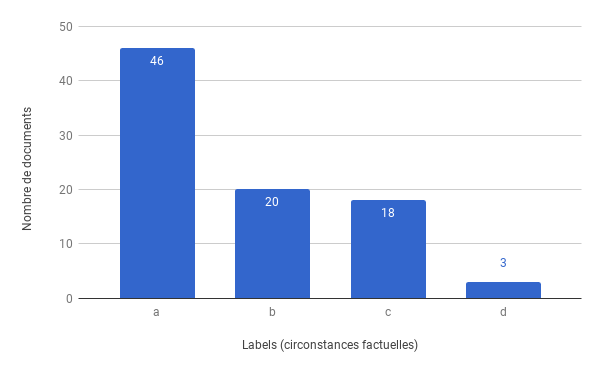
\includegraphics[scale=0.5]{arcpa-data-distrib.png}
%	\caption{Répartition des documents annotés par circonstances factuelles (\textit{arcpa}).}\label{fig:similarite:arcpa-data-distrib}
%\end{figure}

Les terminologies des différents cas se distinguent bien (Tableau \ref{tab:similarite:terminologie-resp_avocat}), et par conséquent, une représentation des documents qui mettrait en évidence ces différents termes permettrait de retrouver les circonstances factuelles associées. 
\begin{table}[h]
	\centering \scriptsize
	\begin{tabular}{|l|p{.85\textwidth}|}
		\hline
		\textbf{Corpus} & \textbf{Terminologie} \\ \hline
		\textit{arcpa} & perte de chance, 
		responsabilité civile professionnelle, 
		civile professionnelle, 
		chance d' obtenir, 
		faute de l' avocat, 
		chance, 
		contradictoirement après débats en audience, 
		nécessairement rejet, 
		avocat est tenu, 
		obtenir gain, 
		obtenir gain de cause, 
		responsabilité professionnelle, 
		audience publique et après, 
		publique et après, 
		chances, 
		aucune chance, 
		perte de chance d' obtenir, 
		délibéré statuant publiquement, 
		perdu une chance, 
		fait perdre une chance, 		
		\\ \hline
		\textit{cas a} & obtenir gain
		obtenir gain de cause
		perte de chance
		perdu une chance
		chances
		nécessairement rejet
		chance
		confié la défense
		conseil' attendu
		chances d' aboutir
		appel que ces condamnations
		nécessairement rejet de la demande
		appel que ces condamnations emportent
		emportent nécessairement
		condamnations emportent
		condamnations emportent nécessairement rejet
		condamnations emportent nécessairement
		emportent nécessairement rejet
		projet d' assignation
		toute chance		
		\\ \hline
		\textit{cas b} & avocat au barreau de dijon
		412 du code de procédure
		barreau de dijon
		412 du code
		devoir de compétence
		régularité et d' autre part
		obliger qu' en l' espèce
		emportant pouvoir
		régime de la responsabilité professionnelle
		régularité et d' autre
		représentation en justice lui imposant
		relève de la responsabilité contractuelle
		imposant d' accomplir
		dispositions combinées des articles 411
		avocat est investi
		avocats relève
		responsabilité professionnelle des avocats
		devoir de conseiller la partie
		tous les actes nécessités
		appel et le jugement entrepris		 
		\\ \hline
		\textit{cas c} &avocat rédacteur d' un acte
		qualité de rédacteur d' acte
		rédacteur d' acte
		rédacteur d' un acte
		avocat rédacteur
		7.2 du règlement intérieur
		7.2 du règlement
		article 7.2 du règlement
		article 7.2 du règlement intérieur
		deux parties à la convention
		validité et la pleine
		portée et les incidences
		initiative de conseiller les deux
		initiative de conseiller
		prévisions des parties
		prendre l' initiative de conseiller
		présence et de prendre
		conseiller les deux parties
		conseiller les deux
		convention sur la portée
		\\ \hline
		\textit{cas d} & instances introduites
		chaque mois sous
		référé du 5 mai
		réunies car
		référé renvoyons
		réception du 20 avril 2009
		référés compte
		référé du 22 novembre
		référé du 27 novembre
		obtenir une décision différente
		référés compte tenu
		l. doivent être condamnés
		appartenait aux appelants
		appelant il n' en demeure
		appel relativement à la juridiction
		appel que les dépens
		apparaît constituer
		valoir tous
		66-879 du 29
		66-879 du 29 novembre 1966				 
		\\ \hline
	\end{tabular}

	\textit{20 premiers termes de 1 à 5 mots sélectionnés à l'aide du coefficient de corrélation $ngl$ (cf. \ref{sec:quanta:poids-globaux-superv})}
	\caption{Terminologies  de la catégorie \textit{arcpa}, et de ses circonstances factuelles annotées.}\label{tab:similarite:terminologie-resp_avocat}
\end{table}

Pour l'évaluation non supervisée, les corpus des catégories de demande des chapitres \ref{chap:quanta} et \ref{chap:sensresultat} sont employés en plus pour l'évaluation non-supervisée. Nous les appelons respectivement $\mathcal{D}_{acpa}$, $\mathcal{D}_{concdel}$, $\mathcal{D}_{danais}$,$\mathcal{D}_{dcppc}$, $\mathcal{D}_{doris}$, $\mathcal{D}_{styx}$.

\subsection{Protocole et outils logiciels}
Pour analyser la validité et l'adéquation de la métrique apprise, nous l'entraînons sur la base générée puis nous l'évaluons sur le corpus annoté $\mathcal{D}_{arcpa}$ restreint aux 74 documents n'appartenant qu'à l'un des cas $L = \lbrace a, b, c \rbrace$. Quant à l'efficacité de la métrique apprise, nous l'entraînons sur toutes les données annotées générées. Les documents sont pré-traités avant leur représentation sous forme vectorielle. Ce prétraitement consiste à sectionner les documents (chapitre \ref{chap:structuration}), à n'utiliser que le contenu principal des documents (Litige + Motifs + Dispositif), à mettre en minuscule et lemmatiser ce contenu, puis à éliminer la ponctuation et des mots inutiles (\textit{stop words})  car ils sont généralement indépendants de toute catégorie. Après pré-traitement, les documents ont une taille allant de 208 à 3812 mots dont une moyenne de 1381 mots. Le vocabulaire $W$ utilisé est restreint au mots du corpus original $D$ sur lequel il faut appliquer les regroupements. La représentation vectorielle emploie les modèles de types TF-IDF avec des n-grammes de 1 à 3 mots (pour prendre en compte l'ordre entre les mots) avec des valeurs de poids globaux supervisés ($\chi_2, gss, ig, marascuilo, ngl, rf$) comprises entre 0.95 et 0.15. Les poids globaux ne sont appris sur la discrimination entre les cas $a,b,c$ mais plutôt entre deux corpus $\mathcal{D}_{arcpa}$ (84 documents) et $\mathcal{D}_{\overline{arcpa}}$ (427) i.e. la terminologie de $\mathcal{D}_{arcpa}$.

\subsection{Validité de la distance apprise}
La base d'entraînement $B$ comprend 10 documents synthétiques générés pour chacun des 74 documents n'ayant qu'un seul label (circonstance factuelle). Nous vérifions ici que la métrique respecte les propriétés des distances, et aussi si elle reste normale après l'entraînement. D'après la matrice des distances entre toutes les paires de document de la base annotées $\mathcal{D_{\text{arcpa}}}$ (Figure \ref{fig:similarite:distance_matrix}),  la "non-négativité", l'identité discernable, et la symétrie sont respectée car toutes les valeurs sont non-négative, seule la diagonale est nulle, et la matrice est symétrique. De plus, toutes les distances sont comprises entre 0 et 1, et par conséquent la métrique est normée (donc la similarité est déduite par $Sim_\mathcal{M} = 1 - Dis_\mathcal{M}$).

\begin{figure}[!htb]
	\centering 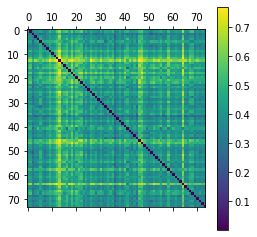
\includegraphics[scale=0.7]{distance_matrix.png}
	\caption{Matrice des distances de la métrique apprise sur $\mathcal{D_{\text{arcpa}}}$}\label{fig:similarite:distance_matrix}
\end{figure}

L'inégalité triangulaire est vérifiée car $Dis_\mathcal{M}(d,d'') - (Dis_\mathcal{M}(d,d') + Dis_\mathcal{M}(d',d'')) \leq 0, \forall (
d,d,d') \in \mathcal{D_{\text{arcpa}}} \times \mathcal{D_{\text{arcpa}}} \times \mathcal{D_{\text{arcpa}}}$ (Figure \ref{fig:similarite:matrice_inegalite_triangulaire}).

\begin{figure}[!htb]
	\centering 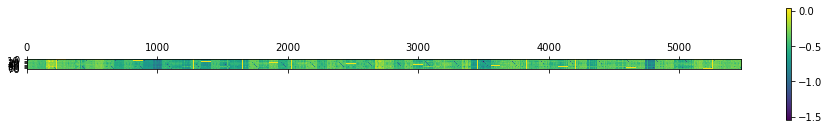
\includegraphics[width=\textwidth]{inegalite_triangulaire.png}
	
	\scriptsize{$Dis_\mathcal{M}(d,d'') - (Dis_\mathcal{M}(d,d') + Dis_\mathcal{M}(d',d'')), \forall (d,d',d'') \in \mathcal{D_{\text{arcpa}}} \times \mathcal{D_{\text{arcpa}}} \times \mathcal{D_{\text{arcpa}}}$, avec les $d$ indicés en lignes et les paires $(d',d'')$ en colonnes.}
	\caption{Matrice de vérification de l'inégalité triangulaire}\label{fig:similarite:matrice_inegalite_triangulaire}
\end{figure}
 


\subsection{Adéquation de la métrique apprise avec le problème}
\label{sec:similarite:adequation}
L'adéquation est mesurée par la formule suivante qui doit tendre vers 0: \[A(Dis) = \sum\limits_{\substack{(l,k) \in L \times L \\ l \neq k}} \sum\limits_{\substack{d \in \mathcal{D}_l \\ d' \in \mathcal{D}_k}} Sim(d,d') + \sum\limits_{l \in L} \sum\limits_{\substack{d \in \mathcal{D}_l \\ d' \in \mathcal{D}_l}} Dis(d,d). \] $L = \lbrace a, b, c \rbrace$ est l'ensemble des labels. Pour tout $l \in L$, $\mathcal{D}_l \subset \mathcal{D}$ désigne le sous-ensemble des documents de $\mathcal{D}$ annotés manuellement avec le label $l$. Cette formule tend vers 0 lorsque la somme des similarités entre documents de labels différents (premier terme) et la somme des distances entre documents de labels égaux (second terme) tendent tous les deux vers 0.
Sur les 74 document annotés, nous obtenons $A(Dis_\mathcal{M}) = 872.635 + 519.151 = 1391.786$ avec une moyenne de similarité entre labels de $0.537$ et de distance entre labels égaux de $0.482$.

L'évaluation des algorithmes de regroupement considèrent parfaite la distance utilisée et la représentation des documents. En considérant les données annotées (regroupement parfait), le coefficient de silhouette peut  permettre d'évaluer les distances. Les valeurs de ce dernier sont ainsi comparées dans le Tableau \ref{tab:similarite:compare-dist-adequation}. La largeur de silhouette étant très proche de 0 et négative pour toutes les distances, les représentations employées pour les documents ne permettent pas d'isoler suffisamment les clusters. Néanmoins, il est possible de trouver une pondération supervisée des termes capable d'améliorée la silhouette, sa valeur devenant même positive pour la distance proposée $Dis_M$ et celle de Manhattan. $Dis_{wmd}$, qui a pourtant la silhouette la plus faible, ne peut pas en profiter car elle n'est pas basée sur un modèle vectoriel.

\begin{table}[!htb]
	\small
	\begin{center}
  \begin{tabular}{|l|c|l|}
  	\hline
  	 & \multicolumn{2}{c|}{\textbf{Silhouette}} \\ 
  	\hline
	\textbf{Distance} & \textbf{ base$^{(*)}$}  & \textbf{modèles vectoriels supervisés$^{(**)}$} \\ \hline
	$Dis_\mathcal{M}$ &-0.007& 0.003 (ATF-NGL) \\ \hline
	$Dis_{braycurtis}$ &-0.005& -0.001 (TF-NGL)\\ \hline
	$Dis_{cos}$ &-0.010& -0.007 (ATF-RF)\\ \hline
	%$Dis_{soft-cos}$ && \\ \hline
	$Dis_{manhattan}$ &-0.014& 0.005 (ATF-NGL) \\ \hline
	$Dis_{euclidienne}$ &-0.005& -0.001 (LOGTF-NGL)  \\ \hline
	$Dis_{jaccard}$ &-0.006& -0.002 (LOGTF-NGL) \\ \hline
	$Dis_{pearson}$ &-0.012& -0.005 (ATF-RF)\\ \hline
	$Dis_{wmd}$  &-0.029& -\\ \hline	
  \end{tabular}
\end{center}
\scriptsize
(*) modèle basé sur les plongements sémantiques de mots pour $Dis_{wmd}$, et modèle TF-IDF pour les autres

(**) modèles vectoriels basés sur la terminologie de la catégorie de demande $arpa$

	\caption{Silhouettes sur le corpus annotée pour différentes distances.} \label{tab:similarite:compare-dist-adequation}
\end{table}

\subsection{Capacité à retrouver les cas annotés manuellement}
%Comparer la vectorisation du document sur tout son contenu vs. sur la restriction aux énoncés de demande de la catégorie (du type "constater", "dire et juger") vs restriction aux conclusions (le raisonnement des parties décrits les circonstances factuelles) + motifs sur la catégorie

%avec choix du nombre de clusters

L'objectif ici est d'obtenir un partitionnement disjoint avec les algorithmes \textit{k-means} et \textit{k-medoids} qui ressemble au mieux à l'annotation manuelle. Le corpus $\mathcal{D}_{arcpa}$ est restreint aux 74 documents annotés des cas $L = \lbrace a, b, c \rbrace$. Le  nombre de clusters $K$ est fixé par conséquent à 3. Le Tableau \ref{tab:similarite:compare-dist-tfidf} présente les scores de validation enregistrés pour chaque distance sur des représentations de base (à base de plongements de mots pour $Dis_{wmd}$, et le modèle TF-IDF pour les autres). Comme sur le regroupement manuel (\ref{sec:similarite:adequation}), les coefficients de silhouette restent très proches de 0 pour toutes les distances, tout comme les valeurs de ARI  et NMI. Par conséquent le regroupement est considéré similaire à un regroupement aléatoire. Néanmoins, $Dis_{pearson}$ et $Dis_{manhattan}$ donnent les meilleurs regroupements avec respectivement le \textit{k-medoids} et le \textit{k-means} (F1-mesure). Comparativement avec les données annotées, les valeurs des différentes métriques de validation restent très faibles. 

Les scores des Tableaux \ref{tab:similarite:compare-dist-silhouette}, et \ref{tab:similarite:compare-dist-wcss} concernent la sélection des valeurs optimale d'hyper-paramètres (algorithme, poids local et global) selon la silhouette  et le critère de cohésion WCSS respectivement. L'objectif est de choisir le critère de validation interne dont la valeur maximale S pour la silhouette ou minimal pour WCSS traduirait une valeur la plus élevée possible des critères externes. Dans l'ensemble, la valeur maximale observée de F1-mesure est 0.558, celle de ARI est 0.180, et celle du NMI est 0.237. Ces valeurs ne correspondent cependant pas aux valeurs optimales de silhouette ou de WCSS (la F1 max est obtenue pour une silhouette nulle par exemple). On observe néanmoins que ces critères pénalisent plus le ARI et le NMI, que la F1, et que le meilleur critère n'est pas le même pour toutes les distances. La distance $Dis_{\mathcal{M}}$ proposée dans ce chapitre parvient à la F1-score maximal pour la valeur minimal de WCSS, de même que $Dis_{pearson}$ pour le max de la silhouette. Nous ne disposons pas malheureusement, de corpus annotée sur d'autres catégories de demande, pour généraliser ces observations et en tirer une conclusion. Néanmoins, le meilleur critère sur la F1-mesure sur le corpus annoté $arcpa$ pour chaque distance est utilisé ci-dessous pour déterminer les valeurs optimales des hyper-paramètres sur les corpus non-annotés i.e. $WCSS_{max}$ pour $Dis_{\mathcal{M}}$, et la $S_{max}$ pour les autres.

\begin{table}[!htb] % TF-IDF
	\scriptsize\centering
	\begin{tabular}{|l||c|c||c|c|c||c||l|}
		\hline
		Distance & ARI & NMI & Précision & Rappel & F1-mesure & Silhouette & Algorithme\\ \hline
		
		
		\multirow{2}{*}{$Dis_\mathcal{M}$} & 0.008$\pm$0.035 & 0.027$\pm$0.018 & 0.437$\pm$0.042 & 0.561$\pm$0.123 & 0.483$\pm$0.039 & 0.011$\pm$0.007 & k-means \\
		 & -0.019 & 0.003 & 0.463 & 0.412 & 0.436 & 0.005 & kmedoids \\ \hline
		
		
		\multirow{2}{*}{$Dis_{braycurtis}$} & 0.004$\pm$0.023 & 0.022$\pm$0.014 & 0.446$\pm$0.055 & 0.490$\pm$0.080 & 0.463$\pm$0.052 & 0.012$\pm$0.006 & k-means \\
		 & 0.027 & 0.041 & 0.415 & 0.353 & 0.382 & 0.004 & kmedoids \\ \hline
		
		\multirow{2}{*}{$Dis_{cos}$} & 0.013$\pm$0.022 & 0.030$\pm$0.021 & 0.446$\pm$0.036 & 0.479$\pm$0.079 & 0.458$\pm$0.038 & 0.016$\pm$0.005 & k-means \\
		 & 0.016 & 0.025 & 0.419 & 0.397 & 0.408 & -0.001 & kmedoids \\ \hline
		
		%\multirow{2}{*}{$Dis_{soft-cos}$}  &&&&&&&  \\  
		 %&&&&&&&  \\ \hline  		
		
		\multirow{2}{*}{$Dis_{manhattan}$} & -0.009$\pm$0.020 & 0.035$\pm$0.019 & 0.481$\pm$0.057 & \textbf{0.627$\pm$0.153} & 0.536$\pm$0.069 & -0.006$\pm$0.012 & k-means \\
		 & -0.029 & 0.022 & 0.463 & 0.511 & 0.486 & -0.006 & kmedoids \\ \hline
		
		\multirow{2}{*}{$Dis_{euclidienne}$} & 0.009$\pm$0.027 & 0.033$\pm$0.022 & 0.445$\pm$0.042 & 0.492$\pm$0.107 & 0.461$\pm$0.049 & 0.017$\pm$0.006 & k-means \\
		 & 0.016 & 0.025 & 0.419 & 0.397 & 0.408 & -0.001 & kmedoids \\ \hline
		
		\multirow{2}{*}{$Dis_{jaccard}$} & 0.011$\pm$0.029 & 0.027$\pm$0.019 & 0.442$\pm$0.044 & 0.487$\pm$0.083 & 0.460$\pm$0.047 & \textbf{0.019$\pm$0.005} & k-means \\
		 & 0.016 & 0.025 & 0.419 & 0.397 & 0.408 & -0.001 & kmedoids \\ \hline
		
		\multirow{2}{*}{$Dis_{pearson}$} & 0.019$\pm$0.028 & 0.032$\pm$0.023 & 0.441$\pm$0.044 & 0.510$\pm$0.098 & 0.468$\pm$0.045 & 0.018$\pm$0.006 & k-means \\
		 & -0.016 & 0.004 & 0.503 & 0.451 & 0.475 & 0.008 & kmedoids \\ \hline
		
		
		$Dis_{wmd}$   & -0.015 & 0.059 & 0.427 & 0.404 & 0.415 & -0.001 & kmedoids \\ \hline
		
	\end{tabular}

	\textit{(moyenne $\pm$ écart-type sur 10 exécutions)}
	\caption{Efficacité des distances à retrouver les 3 cas $a,b,c$ (représentation de base des documents)}\label{tab:similarite:compare-dist-tfidf}
\end{table}

\begin{table}[!htb]
	\scriptsize
	\begin{center}		
	\begin{tabular}{|l|l|l|l|c|c|c|c|c|c|c|c|}%"algorithm","K","lw","gw","s","wcss","ARI","NMI","AMI","P","R","F1"
		\hline
		Distance & Algorithme& K& lw& gw& S$_{max}$ & WCSS & ARI& NMI& P& R& F1 \\ \hline
		$Dis_\mathcal{M}$ & kmeans & 3 & TP & MARASCUILO & 0.172 & 15.654 & -0.004 & 0.032 & 0.396 & 0.356 & 0.374 \\ \hline
		braycurtisDistance & kmeans & 3 & TP & CHI2 & 0.308 & 16.689 & -0.007 & 0.099 & 0.397 & 0.472 & 0.426 \\ \hline
		cosineDistanceNorm & kmeans & 3 & LOGAVE & CHI2 & 0.323 & 1.567 & 0.039 & 0.100 & 0.424 & 0.380 & 0.400 \\ \hline
		euclideanDistance & kmeans & 3 & LOGAVE & CHI2 & 0.252 & 35.305 & 0.010 & 0.078 & 0.405 & 0.397 & 0.398 \\ \hline
		jaccardDistance & kmeans & 3 & LOGAVE & MARASCUILO & 0.329 & 4.713 & 0.049 & 0.039 & 0.420 & 0.603 & 0.491 \\ \hline
		manhattanDistance & kmeans & 3 & ATF & CHI2 & 0.273 & 2103.432 & 0.002 & 0.080 & 0.401 & 0.407 & 0.401 \\ \hline
		pearsonDistance & kmeans & 3 & ATF & MARASCUILO & 0.374 & 5.915 & 0.067 & 0.043 & 0.425 & 0.714 & 0.533 \\ \hline
	\end{tabular}

	\textit{(moyenne sur 10 exécutions)}
\end{center}
	
	S = silhouette, P = précision, R = rappel, F1 = F1-mesure
	
	lw = poids local, gw = poids global

	\caption{Efficacité des distances à retrouver les 3 cas $a,b,c$ (largeur maximale de la silhouette)}\label{tab:similarite:compare-dist-silhouette}
\end{table}


\begin{table}[!htb]
	\scriptsize
	\begin{center}		
		\begin{tabular}{|l|l|l|l|c|c|c|c|c|c|c|c|}%"algorithm","K","lw","gw","s","wcss","ARI","NMI","AMI","P","R","F1"
			\hline
			Distance & Algorithme& K& lw& gw& S & WCSS$_{min}$ & ARI& NMI& P& R& F1 \\ \hline
			$Dis_\mathcal{M}$ & kmedoids & 3 & LOGAVE & NGL & -0.000 & 4.585 & -0.027 & 0.029 & 0.390 & 0.927 & 0.549 \\ \hline
			braycurtisDistance & kmedoids & 3 & ATF & MARASCUILO & -0.015 & 4.949 & -0.003 & 0.030 & 0.396 & 0.331 & 0.361 \\ \hline
			cosineDistanceNorm & kmedoids & 3 & ATF & MARASCUILO & 0.004 & 0.341 & 0.005 & 0.049 & 0.402 & 0.347 & 0.372 \\ \hline
			euclideanDistance & kmedoids & 3 & ATF & MARASCUILO & -0.015 & 15.019 & 0.014 & 0.039 & 0.408 & 0.370 & 0.388 \\ \hline
			jaccardDistance & kmeans & 3 & ATF & MARASCUILO & 0.321 & 3.858 & 0.034 & 0.037 & 0.415 & 0.534 & 0.461 \\ \hline
			manhattanDistance & kmedoids & 3 & ATF & MARASCUILO & 0.033 & 449.012 & 0.044 & 0.060 & 0.428 & 0.372 & 0.398 \\ \hline
			pearsonDistance & kmeans & 3 & LOGTF & IG & 0.131 & 5.231 & 0.017 & 0.057 & 0.411 & 0.358 & 0.382 \\ \hline
		\end{tabular}
		
		\textit{(moyenne sur 10 exécutions)}
	\end{center}
	
	S = silhouette, P = précision, R = rappel, F1 = F1-mesure
	
	lw = poids local, gw = poids global
	
	
	\caption{Efficacité des distances à retrouver les 3 cas $a,b,c$ (WCSS minimal)}\label{tab:similarite:compare-dist-wcss}
\end{table}

\subsection{Evaluation non supervisée des algorithmes sur les 7 catégories de demandes}

%\subsection{Comparaison des zones et représentation vectorielle}

\section{Conclusion}
\label{sec:similarite:conclusion}
Il aurait été judicieux d'augmenter au préalable le volume des corpus par la détection de la présence de catégorie par classification de documents, étant donnée qu'elle est triviale pour les algorithmes traditionnels.